% !TeX root = ../tesis.tex
%%%%%%%%%%%%%%%%%%%%%%%%%%%%%%%%%%%%%%%%%%%%%%%%%%%%%%%%%%%%%%%%%%%
% SECCIÓN 4.2 — VFTModel: Vanishing Fig-Tree Model
%%%%%%%%%%%%%%%%%%%%%%%%%%%%%%%%%%%%%%%%%%%%%%%%%%%%%%%%%%%%%%%%%%%

% =============================================================================
%  4.2 — VISIÓN GENERAL
% =============================================================================
\section{VFTModel: El Motor Analítico de la Red}
\label{sec:vftmodel-intro}

\textbf{VFTModel} (\termino{Vanishing Fig-Tree Model}) es el segundo componente
de la arquitectura de código de esta investigación. Si \textbf{Apimetro} cumple
la función de fuente de datos —exponiendo la geometría de la red de transporte
mediante una \api{} \textsc{rest}—, VFTModel es el \textbf{motor analítico}
que consume esos datos, los transforma en una estructura matemática de grafos y
ejecuta los algoritmos que producen los indicadores topológicos presentados en
el Capítulo~\ref{ch:resultados-vft}.

\begin{figure}[htbp]
  \centering
  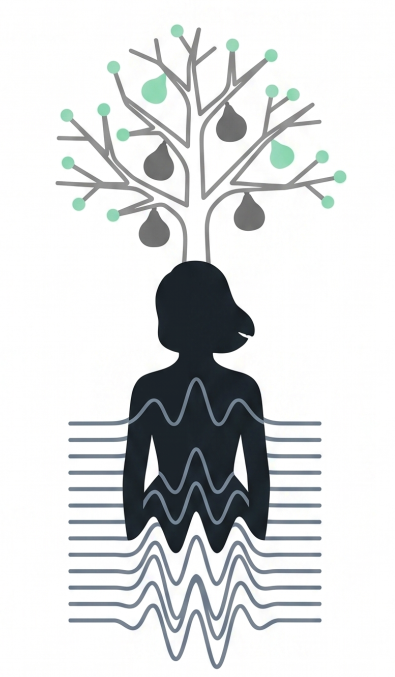
\includegraphics[width=0.45\textwidth]{Figures/Cap4/VFTLogo1.png}
  \caption[Ícono Personal de VFTModel]{Ícono Creado para el proyecto VFTModel}
  \label{fig:VFTModel-icon}
  \fuentefigura{Elaboración propia.}
\end{figure}


\subsection{Contexto y Motivación}
\label{subsec:vft-contexto}

La \zmvm{} alberga una de las redes de transporte público más heterogéneas del
mundo: desde el Metro, que opera en vías exclusivas subterráneas a velocidades
comerciales de hasta 36~km/h, hasta los Corredores Concesionados que comparten
carril con el automóvil particular y absorben la saturación vial de la ciudad.
Esta diversidad opera simultáneamente como fortaleza y como desafío analítico.
Contabilizar kilómetros de línea o número de estaciones no es suficiente para
determinar si la red es eficiente: un sistema puede tener muchas estaciones y
aun así obligar a sus usuarios a recorrer trayectos tortuosos, o concentrar
toda la conectividad en grandes nodos de transbordo mientras las zonas
periféricas
quedan sin alimentación capilar adecuada.

VFTModel nace como respuesta a esta necesidad: un motor analítico reproducible,
de código abierto y matemáticamente fundamentado, capaz de cuantificar la
eficiencia estructural de la red mediante indicadores topológicos derivados de
la teoría de grafos \citep{newman2010networks}. El modelo transforma los
datos geográficos del sistema metropolitano en una estructura matemática de
nodos
y aristas sobre la cual aplica algoritmos de análisis de redes, produciendo
métricas concretas y comparables que permiten evaluar la conectividad del
sistema
e identificar nodos vulnerables.

\subsection{El Nombre: Vanishing Fig-Tree}
\label{subsec:vft-nombre}

La denominación \termino{Vanishing Fig-Tree} —árbol de higuera en desaparición o
Modelo de la Higuera Evanescente— es una metáfora del comportamiento topológico
de una red de transporte fragmentada.
\\
\termino{Vanishing Fig-Tree Model} se basa en dos referencias clave en
diferentes ámbitos:
una es literaria y describe la desesperanza de una situación crítica ante una
decisión
tan trascendente, mientras que la otra describe de manera lírica el llamado
\termino{Punto de No Retorno}:

\citaclave{
  \begin{center}
``From the tip of every branch, like a fat purple fig, a wonderful future
beckoned and
winked. One fig was a husband and a happy home and children, and another fig was
a famous
poet and another fig was a brilliant professor, and another fig was Europe and
Africa and
South America, and another fig was Constantine and Socrates and Attila and a
pack of other
lovers with queer names and offbeat professions, and another fig was an Olympic
lady crew
champion, and beyond and above these figs were many more figs I couldn't quite
make out.
    \\ \vspace{1ex}
I saw myself sitting in the crotch of this fig tree, starving to death, just
because
I couldn't make up my mind which of the figs I would choose. I wanted each and
every
one of them, but choosing one meant losing all the rest, and, as I sat there,
unable
to decide, the figs began to wrinkle and go black, and, one by one, they plopped
    to the ground at my feet.'' 
    
    \vspace{1.5ex}
    \hrule
    \vspace{1.5ex}
    
``De la punta de cada rama, como si de un grueso higo morado se tratara, pendía
un
maravilloso futuro, señalado y rutilante. Un higo era un marido y un hogar feliz
e
hijos y otro higo era un famoso poeta, y otro higo era un brillante profesor, y
otro
higo era Europa y África y Sudamérica y otro higo era Constantino y Sócrates y
Atila
y un montón de otros amantes con nombres raros y profesionales poco usuales, y
otro
higo era una campeona de equipo olímpico de atletismo, y más allá y por encima
de
    aquellos higos había muchos más higos que no podía identificar claramente.
    \\ \vspace{1ex}
Me vi a mí misma sentada en la bifurcación de ese árbol de higos, muriéndome de
hambre sólo porque no podía decidir cuál de los higos escoger. Quería todos y
cada
uno de ellos, pero elegir uno significaba perder el resto, y, mientras yo estaba
allí
sentada, incapaz de decidirme, los higos empezaron a arrugarse y a tornarse
negros y,
    uno por uno, cayeron al suelo, a mis pies.'' \\
    \vspace{1ex}
    \citep{plath2019campana}
  \end{center}
}

\citaclave{
  \begin{center}
    ``My life ain't no holiday \\
    I've been through the point of no return \\
    I've seen what a man can do \\
    I've seen all the hate of a woman too.'' 
    
    \vspace{1.5ex}
    \hrule
    \vspace{1.5ex}
    
    ``Mi vida no es ninguna vacación \\
    He cruzado el punto de no retorno \\
    He visto lo que un hombre puede hacer \\
    También he visto todo el odio de una mujer.'' \\
    \vspace{1ex}
    \citep{neworder_vanishingpoint_1989}
  \end{center}
}

Una higuera no muere cuando pierde sus ramas más delgadas. El tronco y las ramas
principales permanecen, pero su capacidad de expansión y de alimentación colapsa
silenciosamente: las raíces capilares dejan de nutrir las zonas más alejadas, y
el árbol entra en una decadencia progresiva que no es visible desde el exterior
hasta que es demasiado tarde. De manera análoga, una red de transporte puede
mantener sus corredores troncales operativos con plena visibilidad pública,
mientras sus rutas de alimentación capilar desaparecen o se deterioran sin que
ese deterioro aparezca en los indicadores convencionales de pasajeros
transportados o kilómetros de línea. Las zonas que pierden su conexión capilar
quedan aisladas funcionalmente del resto del sistema, aunque sigan figurando en
los mapas oficiales.

El modelo propone medir precisamente esta fragilidad estructural mediante
indicadores que capturen tanto la conectividad interna de los nodos —la
\termino{Fuerza Capilar}— como la eficiencia de los recorridos reales frente a
la distancia teórica mínima —el \termino{Factor de Desviación}—, y el impacto
que tendría la pérdida de un nodo crítico sobre el sistema en su conjunto.

% =============================================================================
%  4.2.2 — ARQUITECTURA
% =============================================================================
\section{Arquitectura del Sistema}
\label{sec:vft-arquitectura}

\subsection{Tres Capas con Responsabilidades Delimitadas}
\label{subsec:vft-capas}

\begin{figure}[htbp]
    \centering
    % Diagrama: Arquitectura Ports-and-Adapters de VFTModel
% Usado en: 4-Capas-Codigo/4-2-VFTModel.tex  (fig:VFTModel-arquitectura)
% Fix 2026-08-28: eliminados actores externos como cajas separadas (diagrama era >18cm);
%   información de sistemas externos integrada dentro de los adaptadores.
\begin{tikzpicture}[
    dominio/.style = {
        rectangle, draw=unamAzul, fill=unamAzul!18,
        text width=3.8cm, align=center,
        minimum height=2.4cm, rounded corners=5pt,
        font=\small\bfseries
    },
    adaptador/.style = {
        rectangle, draw=unamAzul!70, fill=unamAzul!6,
        text width=3.2cm, align=center,
        minimum height=1.8cm, rounded corners=3pt,
        font=\small
    },
    flecha/.style = {Stealth-Stealth, thick, color=unamAzul!55}
]

%% — Dominio central —
\node[dominio] (dom) {
    \textbf{Dominio}\\
    \texttt{src/core/}\\[3pt]
    {\footnotesize Algoritmos \textsc{vft}\\Constructor del grafo}
};

%% — Adaptadores alrededor del dominio —
\node[adaptador, left=0.8cm of dom] (adp-api) {
    \textbf{Adaptador \api{}}\\
    \texttt{src/api/}\\[3pt]
    {\footnotesize FastAPI \textsc{rest} $\cdot$ Go}
};
\node[adaptador, right=0.8cm of dom] (adp-viz) {
    \textbf{Adaptador Viz}\\[3pt]
    {\footnotesize Jupyter $\cdot$ \textsc{qgis}\\Transport-gis}
};
\node[adaptador, below=0.9cm of dom] (adp-per) {
    \textbf{Adaptador Persistencia}\\
    \texttt{src/infrastructure/}\\[3pt]
    {\footnotesize Redis $\cdot$ Celery\\PostgreSQL/PostGIS}
};

%% — Flechas entre adaptadores y dominio —
\draw[flecha] (adp-api) -- (dom);
\draw[flecha] (dom)     -- (adp-viz);
\draw[flecha] (dom)     -- (adp-per);

%% — Borde Docker (en fondo) —
\begin{scope}[on background layer]
    \node[draw=unamAzul!35, dashed, rounded corners=8pt, fill=unamAzul!3,
          fit={(adp-api)(adp-viz)(adp-per)(dom)},
          inner sep=16pt] (docker) {};
\end{scope}

%% — Etiqueta Docker centrada en la parte superior —
\node[font=\scriptsize\bfseries\color{unamAzul!65}, anchor=north]
    at (docker.north) {Docker};

\end{tikzpicture}

    \caption[Arquitectura \textit{Ports and Adapters} de VFTModel]{Diagrama de la
    arquitectura \termino{Ports and Adapters} de VFTModel. El Dominio central
    (\texttt{src/core/}) contiene los algoritmos topológicos y permanece aislado
    de las tecnologías externas. Los tres adaptadores gestionan la comunicación
    con actores externos: API REST, herramientas de visualización y capa de
    persistencia. Todo el sistema corre dentro de un contenedor Docker.}
    \label{fig:VFTModel-arquitectura}
    \fuentefigura{Elaboración propia.}
\end{figure}

VFTModel está organizado bajo el patrón de \termino{arquitectura hexagonal}
(\termino{Ports and Adapters}). La idea central es que el núcleo matemático del
sistema —los algoritmos que calculan los indicadores topológicos— no debe
depender
de cómo lleguen los datos ni de cómo se presenten los resultados. Esta
independencia se logra separando el código en tres capas concéntricas:

\begin{description}
    \item[\textbf{Capa de \api{}} (\texttt{src/api/})]
    Recibe las peticiones \textsc{http}, valida los datos de entrada mediante
    contratos de tipo estrictos y devuelve respuestas \textsc{json}. Es la única
    capa visible para quien consume el sistema desde el exterior.

    \item[\textbf{Capa de Dominio} (\texttt{src/core/})]
    Contiene los algoritmos topológicos, los modelos matemáticos y los servicios
    de construcción del grafo. Aquí reside toda la inteligencia analítica del
    modelo. No depende de cómo lleguen los datos ni de cómo se muestren.

    \item[\textbf{Capa de Infraestructura} (\texttt{src/infrastructure/})]
    Gestiona los clientes \textsc{http} para comunicarse con Apimetro, el acceso
    a archivos \geojson{} locales de respaldo y las colas de procesamiento
    asíncrono. Se encarga de obtener los datos, no de analizarlos.
\end{description}

La Figura~\ref{fig:vft-arquitectura} ilustra la jerarquía de las tres capas y
el sentido de las dependencias entre ellas.

\begin{figure}[H]
    \centering
    % Diagrama: Arquitectura hexagonal de tres capas de VFTModel
% Usado en: 4-Capas-Codigo/4-2-VFTModel.tex  (fig:vft-arquitectura)
\begin{tikzpicture}[
    capa/.style = {
        rectangle, draw=unamAzul, rounded corners=5pt,
        text width=11cm, align=left,
        minimum height=1.6cm, inner sep=10pt
    },
    flecha/.style = {Stealth-Stealth, thick, color=unamAzul!55}
]
    \node[capa, fill=unamAzul!5] (api) {
        \textbf{Capa de \api{}} \hfill \texttt{src/api/}\\
        {\small Peticiones \textsc{http} · Validación Pydantic · Respuestas \textsc{json}}
    };
    \node[capa, fill=unamAzul!12, below=0.45cm of api] (core) {
        \textbf{Capa de Dominio} \hfill \texttt{src/core/}\\
        {\small Algoritmos topológicos · Modelos matemáticos · Constructor del grafo}
    };
    \node[capa, fill=unamAzul!22, below=0.45cm of core] (infra) {
        \textbf{Capa de Infraestructura} \hfill \texttt{src/infrastructure/}\\
        {\small Clientes \textsc{http} · Archivos \geojson{} locales · Colas asíncronas}
    };
    \draw[flecha] (api)  -- (core);
    \draw[flecha] (core) -- (infra);
\end{tikzpicture}

    \caption[Arquitectura hexagonal de VFTModel]{Las tres capas de la arquitectura
    hexagonal de VFTModel. Las flechas bidireccionales indican dependencias
    controladas: cada capa solicita servicios a la inferior; la inferior nunca
    dicta qué calcular a las superiores.}
    \label{fig:vft-arquitectura}
    \fuentefigura{Elaboración propia.}
\end{figure}

El beneficio práctico de esta separación es la reproducibilidad: si el formato
de datos de Apimetro cambia, o si los resultados se requieren en un visor
cartográfico distinto, solo se modifica la capa correspondiente sin alterar el
núcleo matemático.

\subsection{Flujo de Procesamiento}
\label{subsec:vft-flujo}

El procesamiento de una solicitud de análisis sigue una cadena de seis
transformaciones sucesivas, desde la ingesta de datos geográficos crudos hasta
la entrega de métricas finales, como se esquematiza en la
Figura~\ref{fig:vft-flujo}.

\begin{figure}[H]
    \centering
    \resizebox{\linewidth}{!}{%
    % Diagrama: Flujo de procesamiento de VFTModel (6 etapas encadenadas)
% Usado en: 4-Capas-Codigo/4-2-VFTModel.tex  (fig:vft-flujo)
% Nota: el \resizebox{\linewidth}{!}{...} permanece en el capítulo, envolviendo este \input
\begin{tikzpicture}[
    node distance = 0.5cm and 0.35cm,
    caja/.style = {
        rectangle, draw=unamAzul, fill=unamAzul!7,
        text width=1.95cm, align=center,
        minimum height=1.3cm, rounded corners=4pt,
        font=\small
    },
    flecha/.style = {-Stealth, thick, color=unamAzul!70},
    etiq/.style = {
        font=\scriptsize\itshape, color=gray,
        align=center, text width=1.95cm
    }
]
    \node[caja] (apy) {\textbf{Apimetro}\\{\tiny Go Backend}};
    \node[caja, right=of apy]  (val) {\textbf{Validación}\\{\tiny Pydantic}};
    \node[caja, right=of val]  (grf) {\textbf{Constructor}\\{\tiny del Grafo}};
    \node[caja, right=of grf]  (imp) {\textbf{Impedancia}\\{\tiny Motor VFT}};
    \node[caja, right=of imp]  (ana) {\textbf{Analizadores}\\{\tiny Topológicos}};
    \node[caja, right=of ana]  (res) {\textbf{Resultados}\\{\tiny JSON / CSV}};

    \node[etiq, below=0.18cm of apy]  {Estaciones\\y Líneas\\\geojson{}};
    \node[etiq, below=0.18cm of val]  {Contratos\\de datos};
    \node[etiq, below=0.18cm of grf]  {Grafo\\NetworkX};
    \node[etiq, below=0.18cm of imp]  {Pesos en\\minutos};
    \node[etiq, below=0.18cm of ana]  {8 Indicadores};
    \node[etiq, below=0.18cm of res]  {{\upshape\api{}} REST};

    \draw[flecha] (apy) -- (val);
    \draw[flecha] (val) -- (grf);
    \draw[flecha] (grf) -- (imp);
    \draw[flecha] (imp) -- (ana);
    \draw[flecha] (ana) -- (res);
\end{tikzpicture}
}%
    \caption[Flujo de procesamiento de VFTModel]{Cadena de transformación de
    VFTModel: desde los datos geográficos crudos de Apimetro hasta los
    indicadores topológicos publicados vía \api{} \textsc{rest}.}
    \label{fig:vft-flujo}
    \fuentefigura{Elaboración propia.}
\end{figure}

% =============================================================================
%  4.2.3 — ENTRADAS Y VALIDACIÓN
% =============================================================================
\section{Entradas y Validación de Datos}
\label{sec:vft-entradas}

\subsection{Formato de Ingesta: GeoJSON}
\label{subsec:vft-geojson}

VFTModel se alimenta de los datos geográficos producidos por Apimetro en formato
\geojson{} \citep{butler2016geojson}. Cada petición devuelve una
\texttt{FeatureCollection} con dos tipos de elementos:

\begin{itemize}
\item \textbf{Estaciones} (campo \texttt{tipo\_entidad} = \texttt{estacion}):
representadas
    como puntos geográficos (\texttt{Point}), con coordenadas GPS y atributos
    operativos —nombre, sistema, jerarquía de transporte, alcaldía y si es un
    nodo \textsc{cetram}—.
\item \textbf{Rutas} (campo \texttt{tipo\_entidad}\allowbreak{} = \texttt{ruta}
): representadas como
    trazos lineales (\texttt{MultiLineString}), con las métricas que el motor de
    impedancia requiere —velocidad operacional, frecuencia de servicio, tipo de
    derecho de vía y sentido de circulación—.
\end{itemize}

Antes de procesar cualquier elemento, VFTModel valida que todos los campos
requeridos existan y sean válidos, como se describe en la siguiente sección.

\subsection{Validación Estricta con Pydantic}
\label{subsec:vft-pydantic}

Cada \texttt{Feature} recibido es sometido a una validación estricta mediante
\textbf{Pydantic}, una biblioteca de Python que verifica que los datos cumplan
exactamente los contratos de tipo definidos en el modelo. Si algún campo es
inválido —por ejemplo, un sistema de transporte no reconocido o un valor de
velocidad negativo—, el sistema lo rechaza antes de que contamine los cálculos.
Este filtro está implementado en \texttt{src/api/schemas/schemas.py}.

El contrato verifica ocho campos críticos: \texttt{sistema} (Enum de 12
valores), \texttt{tipo\_entidad} (\texttt{estacion} o \texttt{ruta}),
\texttt{jerarquia\_transporte}, \texttt{derecho\_de\_via},
\texttt{velocidad\_promedio\_kmh}, \texttt{frecuencia\_minutos},
\texttt{sentido} y \texttt{es\_cetram}. La especificación completa del contrato
de datos se presenta en el Cuadro~\ref{tab:vft-campos-validados} del Anexo~
\ref{anx:vft-validacion}.

\subsection{Catálogo de Sistemas de Transporte}
\label{subsec:vft-sistemas}

VFTModel reconoce exactamente doce sistemas de transporte metropolitano. Cuando
los datos de velocidad o frecuencia no llegan desde Apimetro, el modelo aplica
valores de \termino{fallback} calibrados a la operación real de cada sistema.
Los sistemas estructurales de mayor peso en el análisis son el STC Metro (36
km/h, vía exclusiva), Metrobús (16.3 km/h, vía confinada), Tren Ligero (22 km/h,
vía exclusiva), \textsc{rtp} (14 km/h, vía mixta) y Corredores Concesionados (11
km/h, vía mixta). El catálogo completo con claves de código y parámetros de
\termino{fallback} se presenta en el Cuadro~\ref{tab:vft-sistemas} del Anexo~
\ref{anx:vft-catalogo}.

El tipo de derecho de vía es el parámetro que determina el coeficiente de
fricción aplicado a cada arista del grafo, como se describe en la
Sección~\ref{subsec:vft-cf}.

% =============================================================================
%  4.2.4 — CONSTRUCCIÓN DEL GRAFO
% =============================================================================
\section{Construcción del Grafo Topológico}
\label{sec:vft-grafo}

\subsection{De la Geometría GeoJSON a NetworkX}
\label{subsec:vft-geom-networkx}

El módulo central del sistema es la clase \texttt{\textbf{VFTGraphBuilder}}
\allowbreak{}
(\path{src/core/services/graph_builder.py}), responsable de transformar las
geometrías \geojson{} en un \textbf{dígrafo} representado mediante la
biblioteca \textbf{NetworkX} de Python \citep{hagberg2008networkx}. La
construcción opera en dos fases internas:

\begin{description}
    \item[\textbf{Fase 1 — Registro de estaciones (nodos):}]
    Cada estación del \geojson{} se convierte en un nodo del grafo,
    identificado por sus coordenadas geográficas (longitud, latitud) y
    enriquecido con sus atributos operativos: nombre, sistema de transporte,
    jerarquía, alcaldía y condición de nodo \textsc{cetram}.

    \item[\textbf{Fase 2 — Trazado de rutas (aristas):}]
    Para cada ruta del \geojson{}, el constructor recorre el
    \texttt{MultiLineString} segmento a segmento, acumulando distancia y
    detectando qué estaciones se encuentran sobre el trazo mediante una
    estructura de búsqueda espacial (\termino{KDTree}) con una tolerancia de
    50~m. Por cada par de estaciones consecutivas detectadas, crea una arista
    con la distancia real acumulada a lo largo del trazo —no la distancia en
    línea recta entre las estaciones—. Esta distinción es crítica para sistemas
    como \textsc{rtp} y Corredores Concesionados, cuyos trazos urbanos pueden
    ser hasta un 40~\% más largos que la cuerda directa.
\end{description}
\subsection{Snapping Lógico Geográfico}
\label{subsec:vft-snapping}

En el modo de integración realista (\texttt{REALISTIC\_INTEGRATION}), el
constructor agrega aristas adicionales de \textbf{transbordo peatonal} entre
estaciones de distintos sistemas que se encuentran dentro de una distancia
configurable. Este proceso —denominado \termino{Snapping Lógico Geográfico}—
representa el comportamiento real del pasajero, que puede caminar de una
estación a otra aunque no estén formalmente conectadas en los datos oficiales.

% --- BLOQUE DE IMÁGENES DEL PROCESO DE SNAPPING ---
\begin{figure}[H]
    \centering
    \begin{subfigure}[b]{0.32\textwidth}
        \centering
        \includegraphics[width=\textwidth]{Figures/Cap4/SnappingProcess1.png}
        \caption{Nodos aislados}
        \label{fig:snap1}
    \end{subfigure}
    \hfill
    \begin{subfigure}[b]{0.32\textwidth}
        \centering
        \includegraphics[width=\textwidth]{Figures/Cap4/SnappingProcess2.png}
        \caption{Evaluación de umbral}
        \label{fig:snap2}
    \end{subfigure}
    \hfill
    \begin{subfigure}[b]{0.32\textwidth}
        \centering
        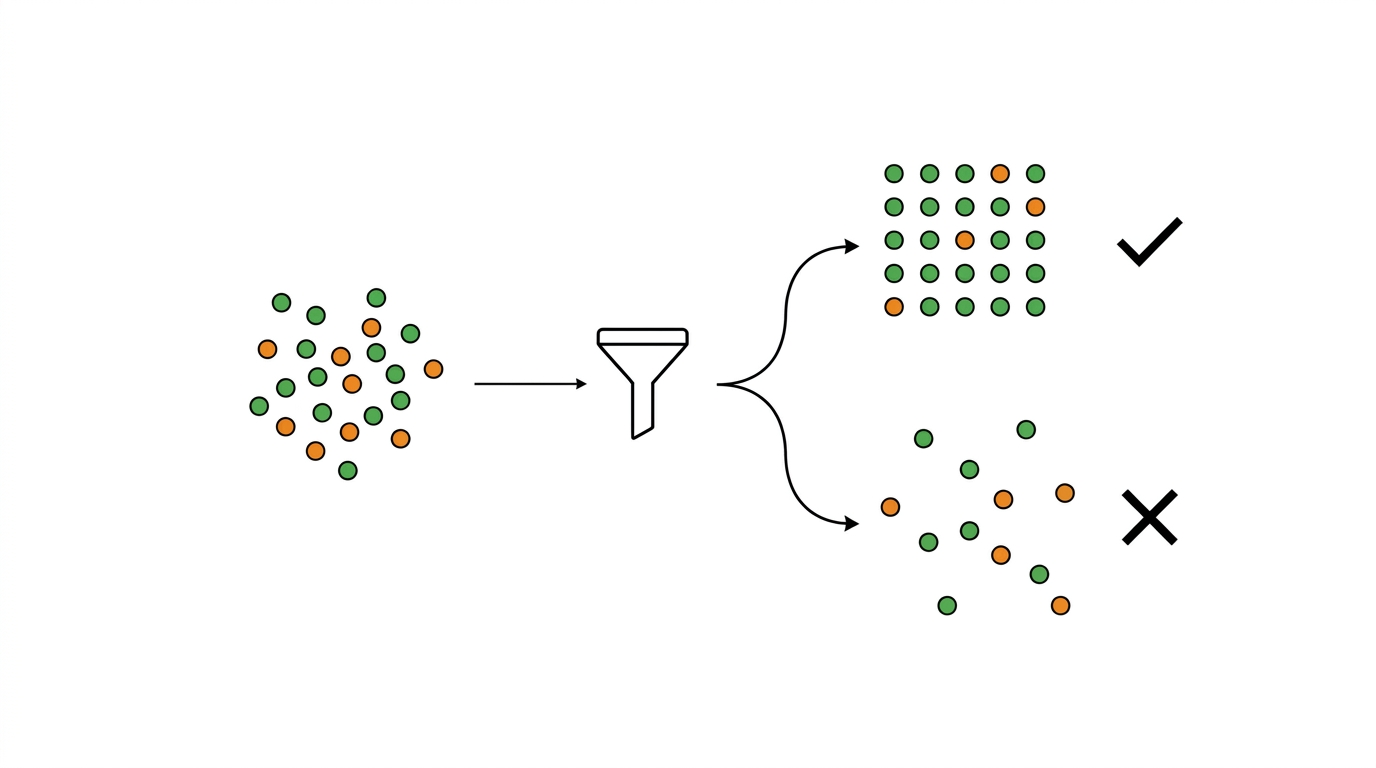
\includegraphics[width=\textwidth]{Figures/Cap4/SnappingProcess3.png}
        \caption{Arista de transbordo}
        \label{fig:snap3}
    \end{subfigure}
    \caption[Secuencia del Snapping Lógico Geográfico]
{Representación visual del proceso de \termino{Snapping Lógico Geográfico}. Las
estaciones
cercanas de distintos sistemas se conectan mediante aristas de transbordo si
cumplen con
    la tolerancia de distancia establecida.}
    \label{fig:proceso-snapping}
    \fuentefigura{Elaboración propia (VFTModel, 2026).}
\end{figure}
% --------------------------------------------------

La tolerancia de transbordo se selecciona a partir de seis umbrales estadísticos
derivados del análisis de las distancias reales entre estaciones de la red
metropolitana, definidos bajo la constante \texttt{STATISTICAL\_THRESHOLDS} en
\texttt{src/core/services/graph\_builder.py}.

\begin{table}[H]
    \centering
    \caption[Umbrales estadísticos de transbordo peatonal en VFTModel]{Umbrales
    estadísticos de tolerancia para el \termino{Snapping Lógico Geográfico}.
El umbral \texttt{Q1} (85~m) es el recomendado para integración conservadora;
    \texttt{Q2} (180~m) integra la mayoría de los \textsc{cetram}s formales.}
    \label{tab:vft-umbrales}
    \begin{tabularx}{\textwidth}{|l|r|X|}
        \hline
        \textbf{Clave} & \textbf{Distancia (m)} & \textbf{Interpretación} \\
        \hline
        \texttt{MIN}  &  15 & Mismo recinto arquitectónico \\
        \texttt{Q1}   &  85 & Transbordo rápido y directo (integración conservadora) \\
        \texttt{Q2}   & 180 & Transbordo promedio real; integra la mayoría de \textsc{cetram}s \\
        \texttt{MEAN} & 245 & Promedio matemático (sesgado por valores atípicos) \\
        \texttt{Q3}   & 420 & Límite máximo de caminata forzada aceptable \\
        \texttt{MAX}  & 880 & Caso atípico; posible falso transbordo \\
        \hline
    \end{tabularx}
    \fuentefigura{Elaboración propia con base en \texttt{graph\_builder.py}
    (VFTModel, 2026).}
\end{table}

El grafo de la \zmvm{} en configuración
\texttt{REALISTIC\_\allowbreak{}INTEGRATION Q1}
resultante contiene \textbf{11{,}115 nodos topológicos} y
\textbf{45{,}679 aristas} —25{,}197 de tránsito y 20{,}482 de transbordo
peatonal generadas algorítmicamente—, tras eliminar 1{,}562 aristas que
superaron el umbral de falsa conexión de 5~km.

Los registros de construcción completos de la corrida del 2026-04-18, que
documentan cada fase del proceso, se presentan en el Anexo~\ref{anx:vft-codigo}.

\subsection{Modos de Operación}
\label{subsec:vft-modos}

\texttt{VFTGraphBuilder} ofrece dos modos de construcción del grafo, que
determinan si se generan o no las aristas de transbordo peatonal:

\begin{description}
    \item[\texttt{STRICT\_TOPOLOGY}:]
    Construye el grafo matemático puro: únicamente las aristas de tránsito
    definidas explícitamente por las rutas del \geojson{}. No agrega conexiones
    entre sistemas distintos. Útil para analizar la topología interna de cada
    línea en aislamiento o para verificar que el grafo refleja exactamente los
    trazos geográficos.

    \item[\texttt{REALISTIC\_INTEGRATION}:]
    Además de las aristas de tránsito, genera las aristas de transbordo peatonal
    entre estaciones próximas de distintos sistemas. El costo de cada arista de
    transbordo incluye el tiempo de caminata (a 5~km/h, límite superior del
    \citep{sedatu2019manual}) más la espera promedio del siguiente servicio
    ($F_v / 2$). Este modo es el utilizado en todos los cálculos de indicadores
    presentados en el Capítulo~\ref{ch:resultados-vft}.
\end{description}

% =============================================================================
%  4.2.5 — MOTOR DE IMPEDANCIA
% =============================================================================
\section{Motor de Impedancia: La Ecuación VFT}
\label{sec:vft-impedancia}

Una vez construido el grafo topológico, el módulo \texttt{VFTImpedanceModel}
(\path{src/core/models/impedance.py}) recorre cada arista y le asigna un
\textbf{peso temporal en minutos}: el tiempo estimado de recorrido que los
algoritmos de caminos mínimos utilizarán para determinar la ruta más eficiente
entre dos estaciones.

\subsection{Distancia Geodésica: Fórmula de Haversine}
\label{subsec:vft-haversine}

Todos los cálculos de distancia del modelo utilizan la \textbf{fórmula de
Haversine}, que obtiene la longitud del arco más corto sobre la superficie de
una esfera entre dos puntos de latitud y longitud conocidos. A diferencia de
la distancia euclidiana plana, Haversine opera sobre coordenadas geográficas
reales y produce metros con un error menor al 0.3~\% para distancias urbanas
dentro de la \zmvm{}.

La fórmula se calcula en dos pasos:

\begin{equation}
    a = \sin^{2}\!\left(\frac{\Delta\varphi}{2}\right)
        + \cos\varphi_1 \cdot \cos\varphi_2
          \cdot \sin^{2}\!\left(\frac{\Delta\lambda}{2}\right)
    \label{eq:haversine-a}
\end{equation}

\begin{equation}
    d = 2R \cdot \arctan2\!\left(\sqrt{a},\;\sqrt{1-a}\right)
    \label{eq:haversine-d}
\end{equation}

\begin{itemize}
    \item $\varphi_1, \varphi_2$: latitudes de los dos puntos en radianes.
    \item $\Delta\varphi = \varphi_2 - \varphi_1$: diferencia de latitudes.
    \item $\Delta\lambda = \lambda_2 - \lambda_1$: diferencia de longitudes.
    \item $R = 6{,}371{,}000$~m: radio medio de la Tierra.
    \item $d$: distancia geodésica resultante en metros.
\end{itemize}

La implementación como método estático de \texttt{VFTImpedanceModel} es
reutilizada por prácticamente todos los módulos del sistema. El código fuente
completo se presenta en el Anexo~\ref{anx:vft-codigo}.

\subsection{Coeficiente de Fricción Vial}
\label{subsec:vft-cf}

El \textbf{Coeficiente de Fricción Vial} ($CF$) traduce el tipo de derecho de
vía de cada segmento en un penalizador multiplicativo sobre el tiempo de
traslado. Se obtiene mediante:

\begin{equation}
    CF = 1 + \alpha \cdot \beta_{\text{ZMVM}}
    \label{eq:vft-cf}
\end{equation}

\begin{itemize}
    \item $\alpha \in \{0.0, 0.2, 0.5, 1.0\}$: factor de exposición al tráfico
    según el tipo de derecho de vía, con referencia normativa en
    \citep{sedatu2019manual}.
    \item $\beta_{\text{ZMVM}} = 0.759$: índice de saturación vial de la
    \zmvm{} (\termino{TomTom Traffic Index}).
\end{itemize}

La clase \texttt{\textbf{FrictionCalculator}} implementa este cálculo de forma
aislada, aplicando el principio de vía mixta ($CF = 1.759$) como caso
conservador por defecto. La implementación Python completa se presenta en el
Anexo~\ref{anx:vft-codigo}.

\subsection{Ecuación VFT: Peso Temporal de Cada Arista}
\label{subsec:vft-ecuacion}

Con la distancia geodésica y el coeficiente de fricción disponibles, el método
\path{apply_impedance()} asigna el peso temporal a cada arista del grafo:

\begin{equation}
    w_{ij} = \frac{d_{ij}}{v_{ij}} \cdot CF_{ij}
    \label{eq:vft-peso}
\end{equation}

\begin{itemize}
    \item $w_{ij}$: peso de la arista en minutos (tiempo de viaje estimado entre
    estaciones $i$ y $j$).
\item $d_{ij}$: distancia real del trazo entre $i$ y $j$ en metros, acumulada
    vértice a vértice sobre el \texttt{MultiLineString} durante la construcción
    del grafo.
    \item $v_{ij}$: velocidad comercial del sistema en metros por minuto:
    $v_{ij} = v_{\text{km/h}} \times (1000/60)$.
    \item $CF_{ij}$: Coeficiente de Fricción Vial de la arista
    (Ecuación~\ref{eq:vft-cf}).
\end{itemize}

La implementación Python del método \path{apply_impedance()} se presenta en el
Anexo~\ref{anx:vft-codigo}.

Las aristas de transbordo peatonal quedan excluidas de este proceso porque
ya recibieron su peso durante la construcción del grafo:
$w_{\text{transbordo}} = t_{\text{caminata}} + F_v / 2$ (véase la
Sección~\ref{subsec:res-penalizacion-transferencia} del Capítulo~
\ref{ch:resultados-vft}).
El atributo \texttt{weight} de cada arista —en minutos— es la entrada de todos
los algoritmos de caminos mínimos ejecutados en los indicadores de Fase~3.

% =============================================================================
%  4.2.6 — INDICADORES
% =============================================================================
\section{Indicadores Topológicos Implementados}
\label{sec:vft-indicadores}

VFTModel organiza sus indicadores en cuatro fases de cálculo progresivo,
cuya dependencia es estricta: las Fases~III y IV requieren un grafo
completamente
ponderado —producto de las Fases~I y II— para ejecutar los algoritmos de caminos
mínimos. El Cuadro~\ref{tab:vft-indicadores-estado} presenta el mapa completo
de indicadores con su estado de implementación a la fecha de cierre del
documento.

\begin{table}[H]
    \centering
    \caption[Indicadores topológicos de VFTModel y estado de implementación]{
Indicadores topológicos de VFTModel, sus símbolos y estado de implementación.
    Los resultados de cada indicador se presentan en el
    Capítulo~\ref{ch:resultados-vft}.}
    \label{tab:vft-indicadores-estado}
    \begin{tabularx}{\textwidth}{|c|c|X|l|}
        \hline
        \textbf{Fase} & \textbf{\#} & \textbf{Indicador} & \textbf{Estado} \\
        \hline
        \multirow{4}{*}{\textbf{I}}
          & 1 & Validación de Impedancia                  & Implementado \\
          & 2 & Cobertura Espacial ($C$)                  & Implementado \\
          & 3 & Fuerza Capilar ($FC$)                     & Implementado \\
          & 4 & Factor de Desviación ($DF$)               & Implementado \\
        \hline
        \multirow{3}{*}{\textbf{II}}
          & 5 & Coeficiente de Fricción Vial ($CF$)       & Implementado \\
          & 6 & Penalización por Transferencia ($T_b$)    & Parcial      \\
          & 7 & Node Score ($\text{VFT\_score}$)          & Planificado  \\
        \hline
        \multirow{2}{*}{\textbf{III}}
          & 8 & Tiempo de Viaje Promedio ($T$)            & Pendiente    \\
          & 9 & Centralidad de Intermediación ($B(v)$)   & Pendiente    \\
        \hline
        \textbf{IV}
          & 10 & Vulnerabilidad Estructural ($\Delta E$) & Pendiente    \\
        \hline
    \end{tabularx}
    \fuentefigura{Elaboración propia (VFTModel, 2026-04-28).}
\end{table}

Los indicadores de Fase~I son implementados en módulos independientes dentro de
\path{src/core/algorithms/topologicalIndicators/}: la clase
\texttt{SpatialCoverageAnalyzer} para la cobertura espacial, la clase
\texttt{CapillaryStrengthAnalyzer} para la fuerza capilar, y el submódulo
\texttt{detaurFactor/} —con sus módulos \texttt{engine.py} y
\texttt{orchestator.py}— para el factor de desviación.

% =============================================================================
%  4.2.7 — SALIDAS
% =============================================================================
\section{Salidas: API REST con FastAPI}
\label{sec:vft-salidas}

Los resultados de VFTModel se entregan a través de una
\textbf{\api{} \textsc{rest}}
construida con \textbf{FastAPI}, expuesta localmente en \texttt{localhost:8000}
con documentación interactiva disponible en el endpoint \texttt{/docs}.

La \api{} expone cinco endpoints bajo \texttt{/api/v1/network/}:
\texttt{build-auto} (POST, construye el grafo en caché),
\texttt{spatial-coverage} (GET, cobertura por alcaldía),
\texttt{topological/capillary-strength} (GET, ranking de fuerza capilar),
\texttt{topological/geo-capillary} (GET, macro-hubs) y
\texttt{topological/detour-factor} (GET, factor de desviación por par O-D). La
especificación completa de los endpoints se presenta en el Cuadro~
\ref{tab:vft-endpoints} del Anexo~\ref{anx:vft-api}.

Cada respuesta \textsc{json} puede contener tres tipos de datos:

\begin{itemize}
    \item \textbf{Tablas de métricas:} listas de nodos con su puntuación en el
    indicador calculado, ordenadas de mayor a menor relevancia.
    \item \textbf{Geometrías de ruta:} la trayectoria real sobre la red y la
    línea recta teórica entre origen y destino, ambas en formato \geojson{},
    listas para ser renderizadas en visores cartográficos.
    \item \textbf{Resúmenes estadísticos:} promedio, máximo y distribución del
    indicador sobre el conjunto de pares O-D analizados en el muestreo.
\end{itemize}
